\documentclass{article}
\usepackage[utf8]{inputenc}
\usepackage{tikz}
\usetikzlibrary{trees}

\begin{document}

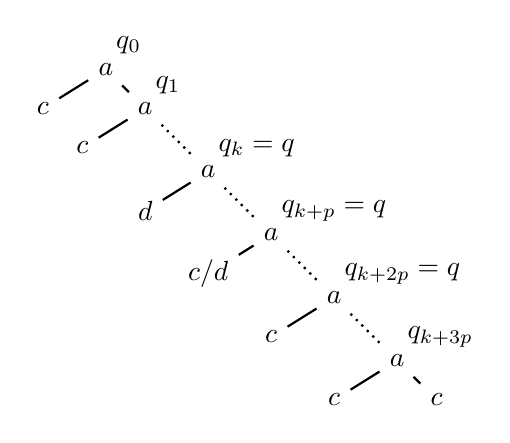
\begin{tikzpicture}[thick]

  \path (0,0)   node (root)    {$a$}    -- +(0,.3) node[right]{$q_0$}
  -- +(-.8,-.5) node (0)       {$c$}
  -- ++(.5,-.5) node (1)       {$a$}    -- +(0,.3) node[right]{$q_1$}
  -- +(-.8,-.5) node (10)      {$c$}
  -- ++(.8,-.8) node (k+1)     {$a$}    -- +(0,.3) node[right]{$q_k=q$}
  -- +(-.8,-.5) node (k+10)    {$d$}
  -- ++(.8,-.8) node (k+p+1)   {$a$}    -- +(0,.3) node[right]{$q_{k+p}=q$}
  -- +(-.8,-.5) node (k+p+10)  {$c/d$}
  -- ++(.8,-.8) node (k+2p+1)  {$a$}    -- +(0,.3) node[right]{$q_{k+2p}=q$}
  -- +(-.8,-.5) node (k+2p+10) {$c$}
  -- ++(.8,-.8) node (k+3p)    {$a$}    -- +(0,.3) node[right]{$q_{k+3p}$}
  -- +(-.8,-.5) node (k+3p0)   {$c$}
  -- ++(.5,-.5) node (k+3p1)   {$c$}
  ;

  \draw[-] (root) edge (0) edge (1)
  (1) edge (10) edge[dotted] (k+1)
  (k+1) edge (k+10) edge[dotted] (k+p+1)
  (k+p+1) edge (k+p+10) edge[dotted] (k+2p+1)
  (k+2p+1) edge (k+2p+10) edge[dotted] (k+3p)
  (k+3p) edge (k+3p0) edge (k+3p1)
  ;

\end{tikzpicture}

\end{document}